\subsection{Classical optimizer}

A wide variety of classical optimizers have been employed within QAOA, as reviewed in the literature~\cite{blekos_review_2024}.  
In this work, we focused on optimizers available in the SciPy library and tested representative classes: bounded vs.\ unbounded and gradient-free vs.\ gradient-based.  

Gradient-free methods such as Nelder-Mead showed promising performance for small problems but scale poorly with the number of parameters, and were therefore discarded. Cobyla exhibited poor convergence and frequent trapping in local minima, even for few-qubit cases, making it unsuitable for this study. Among gradient-based methods, the best performance was obtained with BFGS and its bounded variant L-BFGS-B:

\begin{itemize}
    \item \textbf{L-BFGS-B.}  
    This bounded optimizer is well-suited for QUBO and MaxCut problems, where parameter symmetries justify restricting $\gamma$ and $\beta$ to specific intervals. Under such constraints, L-BFGS-B often produces adiabatic-like parameter trajectories, with $\gamma$ starting near zero and increasing smoothly, while $\beta$ decreases monotonically toward zero.  

    \item \textbf{BFGS.}  
    As an unbounded optimizer, BFGS allows variational parameters to take any real value. In all tested cases up to 8~qubits, BFGS consistently outperformed L-BFGS-B, likely because its unbounded nature helps it escape local minima that trap the bounded optimizer (see Fig.~\ref{fig:optimizer_comparison}).
\end{itemize}

\begin{figure}[h]
    \centering
    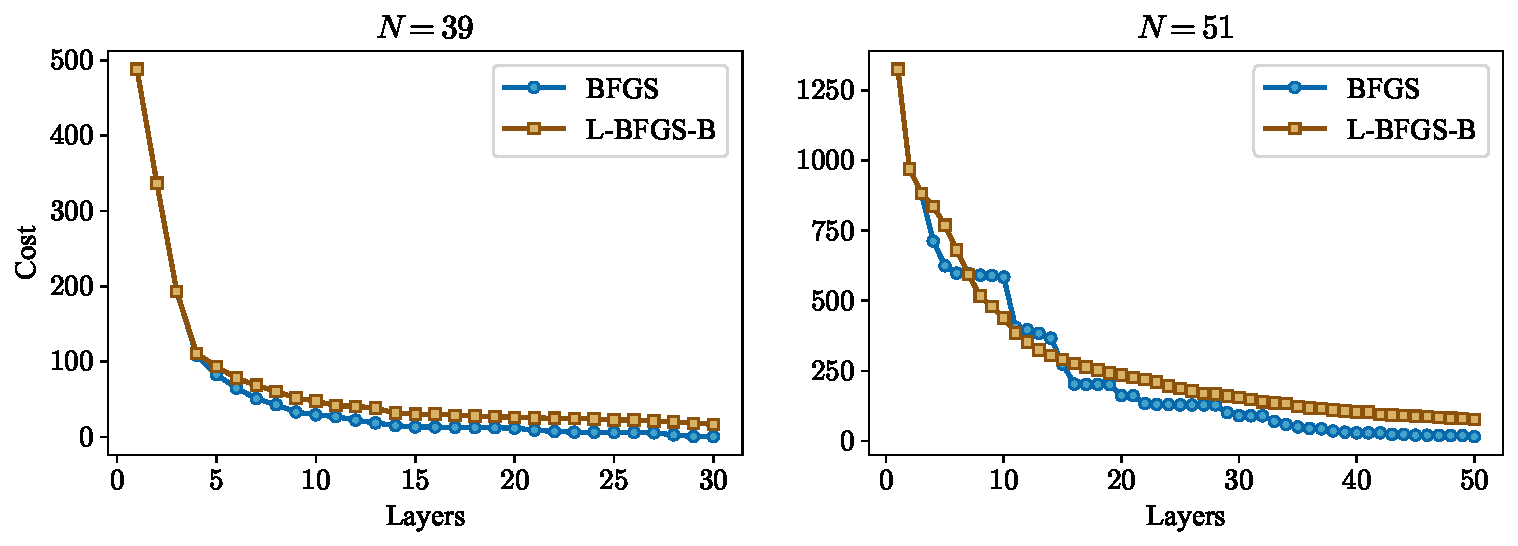
\includegraphics[width=0.99\textwidth]{03-methodology/figs/optimizer_comparison.pdf}
    \caption{Cost evolution comparison between BFGS and L-BFGS-B for factorizing $N=39$ and $N=51$ using the standard protocol. The performance gap was observed consistently up to 8-qubit problems.}
    \label{fig:optimizer_comparison}
    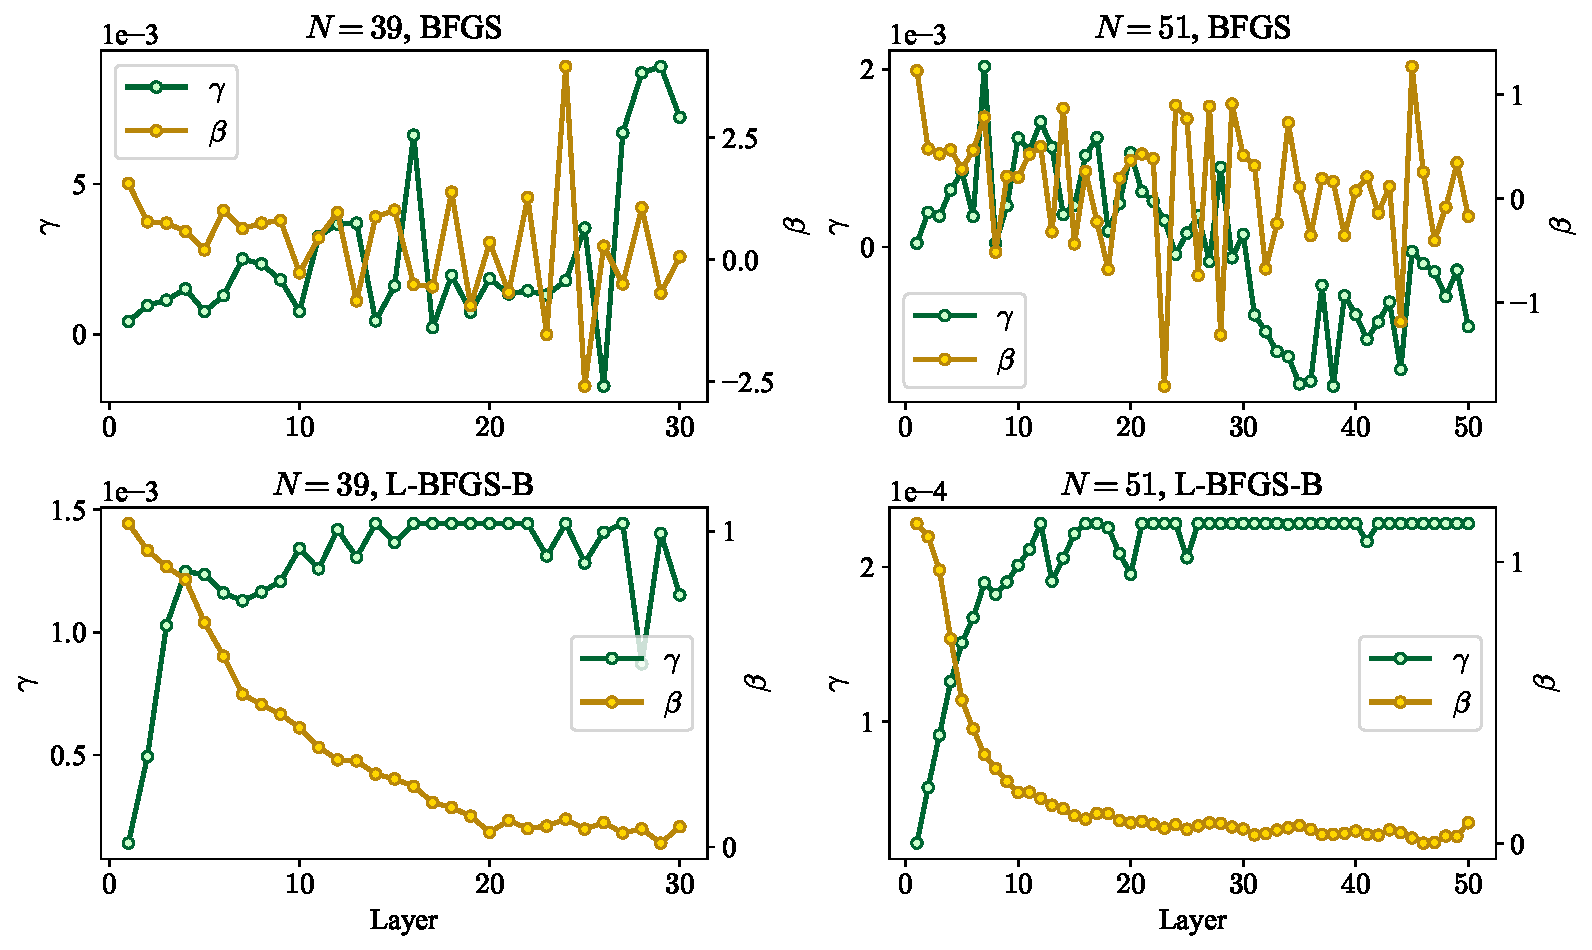
\includegraphics[width=1\textwidth]{03-methodology/figs/optimizer_parameters_comparison.pdf}
    \caption{Variational parameter evolution for $N=39$ and $N=51$ using BFGS and L-BFGS-B. An adiabatic-like trajectory emerges under L-BFGS-B due to parameter bounds.}
    \label{fig:optimizer_parameter_comparison}
\end{figure}

Based on these findings, \textbf{BFGS is selected as the classical optimizer for all experiments}.  
This choice complements the other elements of our QAOA setup, ensuring a consistent and high-performance framework for comparing the standard protocol and the proposed linearized protocol.